\documentclass[letterpaper]{article}
\usepackage[T1]{fontenc}
\usepackage{spconf,amsmath,graphicx,booktabs}
\usepackage{newtxmath}
\usepackage[hidelinks]{hyperref}

\urlstyle{same}
\hypersetup{pdftitle={Validation Speaker Exposure and Checkpoint Selection in Speech Emotion Recognition},pdfauthor={Tian Xie}}
\title{Validation Speaker Exposure and Checkpoint Selection\\in Speech Emotion Recognition}
\name{Tian Xie}
\address{University of Toronto\\tianjack.xie@mail.utoronto.ca}
\begin{document}
\maketitle
\begin{abstract}
Checkpoint selection can change speaker-independent speech emotion recognition results even when training and testing are held fixed. We compare seen- and unseen-speaker validation using cross-entropy (CE) or unweighted average recall (UAR) on shared candidate trajectories and unfamiliar-speaker tests. An original 384-fit study and a separately frozen 720-fit supplement cover three native tasks, two backbones, and longer candidate windows. HuBERT CE selection favors seen-speaker validation by 1.576, 4.018, and 1.398 percentage points on CREMA-D, SUBESCO, and RAVDESS; CE-versus-UAR interactions are supported in the first two tasks. Extending RAVDESS WavLM candidate windows from 15 to 45 epochs increases the CE contrast by 2.257 points. Six of ten supplemental tests survive joint Holm correction. These findings establish criterion- and window-dependent selection effects within the studied programs: validation population, selection metric, and candidate window should be reported together.
\end{abstract}
\begin{keywords}
speech emotion recognition, speaker independence, checkpoint selection, validation, evaluation
\end{keywords}

\section{Introduction}
Speech emotion recognition (SER) is often evaluated on speakers absent from training. SERAB and Antoniou et al. separate training, validation, and test speakers~\cite{serab,antoniou}. Finite-sample selection criteria can also affect evaluation~\cite{cawley}. Validation optimism and selected-model performance are distinct: a larger validation--test gap need not imply a worse model on a common unfamiliar-speaker test.

Prior SER work compares random and actor-independent evaluation across datasets, models, or repeated runs~\cite{ibrahim,zielonka,kumari}; matching training counts across speaker/text conditions also has precedent~\cite{atmaja}. Such comparisons may change training or test membership together with the validation boundary. We hold the training trajectory and outer test fixed, and vary the checkpoint-selection policy: validation on familiar versus unfamiliar speakers, each using CE or UAR. All four policies choose from exactly the same saved models, removing between-run training differences from their comparison.

The contributions are a matched-trajectory comparison separating selected-model performance from validation optimism; a completed 384-fit study and 720-fit supplement testing a second backbone and longer selection windows; and a public numerical artifact retaining all primary outcomes and absolute policy scores~\cite{artifact}. Together, they show why specifying speaker separation alone leaves a consequential part of SER evaluation unspecified.

\section{Experimental design}
\subsection{Shared trajectories and query roles}
Each corpus uses 24 draws and five outer folds. The original program has 360 A-trained main fits and 24 B-trained CREMA-D fold-0 controls. CREMA-D, SUBESCO, and RAVDESS retain six, seven, and eight native classes and 91, 20, and 24 speakers, respectively~\cite{cremad,subesco,ravdess}. Within a draw, metadata hashing partitions speakers into five outer folds stratified by recorded sex; each speaker enters exactly one outer fold. Outside each fold, disjoint development groups A and B have equal sex-balanced quotas. Eligible speakers in each sex stratum are hash-ranked using phase, corpus, draw, and fold identifiers; successive quotas form A and B without model scores. Unused speakers remain excluded.

All query roles share texts disjoint from fit texts (Table~\ref{tab:panels}). Frozen representatives are MD-preferred/otherwise XX for CREMA-D, T1 for SUBESCO, and normal-intensity R1 for RAVDESS, without substitute takes. Outer queries retain available representatives, requiring every native class for each outer speaker. Insufficient development capacity causes metadata failure, not outcome-dependent resampling. Both studies use private pre-execution source/plan freezes, not public preregistration; the corpora have prior research exposure.

\begin{table}[t]
\centering\small
\caption{Per-context allocation. A/B counts are distinct speakers; fit/query counts are recordings. A and B are sex-balanced.}
\label{tab:panels}
\setlength{\tabcolsep}{3pt}
\begin{tabular}{lrrrcrr}\toprule
Corpus & Classes & A/B & Outer & Texts$^a$ & Fit & Query$^b$\\\midrule
CREMA-D & 6 & 24/24 & 17/19 & 4/2 & 576 & 288\\
SUBESCO & 7 & 8/8 & 4 & 4/2 & 224 & 112\\
RAVDESS & 8 & 8/8 & 4/6 & 1/1 & 64 & 64\\\bottomrule
\end{tabular}
\par\raggedright\small
$^a$ Fit/query text counts. $^b$ Each development query role. Outer queries use available CREMA-D representatives, 56 SUBESCO recordings, or 32/48 RAVDESS recordings; slash counts denote different fold sizes.
\end{table}

Main fits train on A; A and B queries provide seen- and unseen-speaker validation. WavLM Base+~\cite{wavlm} and HuBERT Base~\cite{hubert} use native-class linear heads over mean-pooled final features, with only the top four Transformer layers and head trainable. Fixed settings are AdamW, encoder/head learning rates $5\times10^{-5}/10^{-3}$, weight decay .01, batch size 16, and unweighted CE. Every epoch traverses the fit set, without early stopping or hyperparameter search. Training uses FP16 autocast with FP32 parameters; evaluation uses FP32. Mono 16\,kHz audio is silence-trimmed at 30\,dB; training uses three-second crops or zero-padding, and evaluation retains at most ten seconds.

Main A-trained fits record A, B, and outer logits every epoch; original B-trained controls retain only epoch~15. Four rules minimize whole-role mean CE or maximize whole-role native-class macro recall (UAR) on A or B; exact ties select the earliest epoch, using rational recall for UAR ties. This is not average speaker UAR. Each role has separate fixed sorted batches of 16, so outer audio cannot pad validation batches. Mean pooling lacks a length mask: fixed batching preserves padding context without removing padding effects. Outer scores never select epochs or determine training length.

\subsection{Separately frozen backbone and window supplement}
HuBERT trains for 15 epochs on all three corpora (360 fits). New WavLM fits use 15 epochs on CREMA-D and 45 on SUBESCO/RAVDESS (360 fits): 720 trajectories and 18,000 epoch traversals in total. The matrix is not fully factorial; HuBERT 45 and CREMA-D WavLM 45 are absent. Each long trajectory supplies both its own 15- and 45-epoch selection windows, rather than using the original Windows WavLM run as a paired baseline.

The supplement reuses the frozen panels and fit/query order. Within a context, both backbones share head initialization and training/order/crop seed conventions, with a new execution seed domain and a separate crop domain. Backbone and horizon do not enter these seeds. This matches stochastic schedules across models; architecture and pretraining still differ. Both new models run in the same Linux/CUDA environment, unlike the original Windows execution. Eight excluded technical pilots include independent 15-epoch companions whose histories, logits, and selections exactly matched the corresponding 45-epoch prefixes. These checks validate prefix reuse without adding inferential replicates.

\subsection{Estimands and inference}
Let $T(g,q;w)$ be outer UAR (\%) at the epoch selected within window $w$ by group $g$ (seen $s$, unseen $u$) and criterion $q$. Per-context effects are
\begin{align}
\delta_q(w)&=T(s,q;w)-T(u,q;w),\\
J(w)&=\delta_{\rm CE}(w)-\delta_{\rm UAR}(w),\\
L_{\rm CE}&=\delta_{\rm CE}(45)-\delta_{\rm CE}(15),\\
L_J&=J(45)-J(15).
\end{align}
All contrasts are UAR percentage points, not CE losses or validation-optimism differences $\Delta(V-T)$. Positive $\delta$ favors the seen-selected model on the common outer test. Four rules share one candidate trajectory within a model and require no additional training.

Five fold effects are averaged equally per draw. Two-sided one-sample $t$ inference uses 24 draw effects ($df=23$), not 120 independent folds. The original six-test family contains $(\delta_{\rm CE},J)$ in each corpus with Holm6. The new ten-test family jointly contains six HuBERT15 effects and four WavLM window effects, with one Holm10 at .05. Families remain separate; no tests or tails are changed after outcomes. Pointwise 95\% $t$ intervals are not simultaneous intervals or equivalence tests. Undefined zero-variance tests retain NA family slots. Absolute UAR, $\delta_{\rm UAR}$, new WavLM level effects, and paired HuBERT-minus-WavLM15 differences are prespecified descriptions without additional $p$ values.

Inference conditions on these finite corpora, panels, and training programs. Repeated speakers, folds, rules, and the 1,104 total fits do not enlarge the independent sample size. Native tasks differ, so no pooled corpus or language-effect inference is performed. Original whole-training-group exchange controls and post hoc 8/10/12/15-epoch truncations remain descriptive artifact analyses~\cite{artifact}; neither supplies new replication or determines which supplement outcomes are included.

\begin{table*}[t]
\centering\small
\caption{All primary effects in UAR percentage points (pp), pointwise 95\% draw-level $t$ intervals, and two-sided raw/within-family Holm $p$. Panel A uses Holm6; B and C jointly use Holm10. Pointwise intervals are not adjusted for multiplicity.}
\label{tab:primary}
\setlength{\tabcolsep}{5pt}
\begin{tabular}{llrrrr}\toprule
Corpus & Contrast & Mean & Pointwise 95\% CI & Raw $p$ & Holm $p$\\\midrule
\multicolumn{6}{l}{\textit{A. Original WavLM, 15 epochs: six-test family}}\\
CREMA-D & $\delta_{\mathrm{CE}}$ & 0.935 & [0.287, 1.583] & 0.0066 & 0.0264\\
CREMA-D & $J$ & 0.937 & [0.210, 1.663] & 0.0138 & 0.0413\\
SUBESCO & $\delta_{\mathrm{CE}}$ & 2.247 & [0.945, 3.549] & 0.0016 & 0.0083\\
SUBESCO & $J$ & 2.560 & [1.103, 4.016] & 0.0014 & 0.0083\\
RAVDESS & $\delta_{\mathrm{CE}}$ & 0.486 & [-0.198, 1.170] & 0.1549 & 0.3098\\
RAVDESS & $J$ & 0.469 & [-0.633, 1.570] & 0.3877 & 0.3877\\\midrule
\multicolumn{6}{l}{\textit{B. Supplement: HuBERT, 15 epochs (six of ten tests)}}\\
CREMA-D & $\delta_{\rm CE}$ & 1.576 & [1.000, 2.153] & $9.28\!\times\!10^{-6}$ & $7.43\!\times\!10^{-5}$\\
CREMA-D & $J$ & 1.296 & [0.499, 2.093] & 0.0027 & 0.0161\\
SUBESCO & $\delta_{\rm CE}$ & 4.018 & [2.835, 5.201] & $3.67\!\times\!10^{-7}$ & $3.67\!\times\!10^{-6}$\\
SUBESCO & $J$ & 3.616 & [2.332, 4.900] & $6.15\!\times\!10^{-6}$ & $5.54\!\times\!10^{-5}$\\
RAVDESS & $\delta_{\rm CE}$ & 1.398 & [0.425, 2.370] & 0.0068 & 0.0340\\
RAVDESS & $J$ & 0.703 & [-0.510, 1.917] & 0.2428 & 0.4857\\
\midrule
\multicolumn{6}{l}{\textit{C. Supplement: WavLM window 45 minus 15 (four of ten tests)}}\\
SUBESCO & $L_{\rm CE}$ & 0.283 & [-0.009, 0.574] & 0.0567 & 0.1702\\
SUBESCO & $L_J$ & 0.268 & [-0.761, 1.297] & 0.5954 & 0.5954\\
RAVDESS & $L_{\rm CE}$ & 2.257 & [1.294, 3.220] & $6.82\!\times\!10^{-5}$ & $4.77\!\times\!10^{-4}$\\
RAVDESS & $L_J$ & 1.849 & [0.343, 3.355] & 0.0183 & 0.0731\\
\bottomrule
\end{tabular}
\end{table*}

\begin{figure*}[t]
\centering
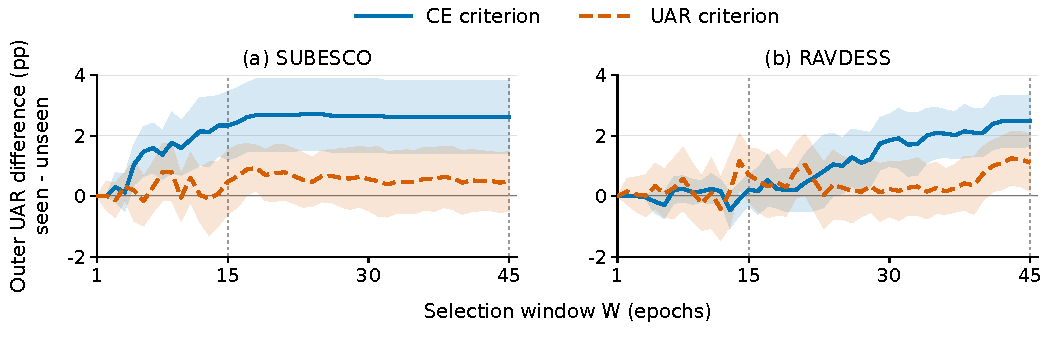
\includegraphics[width=\textwidth]{../figures/window_selection.pdf}
\caption{Post hoc window profiles for supplemental WavLM45. Lines show seen-minus-unseen outer UAR after CE/UAR selection; bands are pointwise 95\% $t$ intervals over 24 five-fold draw means, not simultaneous bands or new tests. W15 uses the same trajectories' prefixes. All fits completed 45 epochs; the axis changes eligible checkpoints, not training termination.}
\label{fig:windows}
\end{figure*}

\section{Results}
\subsection{Original study and second backbone}
Table~\ref{tab:primary} retains both complete inferential families. In the original study, positive CE exposure contrasts and CE-versus-UAR interactions on CREMA-D and SUBESCO survive Holm6; both RAVDESS estimates remain uncertain. No corpus or test was dropped within that original frozen program. The supplement was designed after reviewing those results and frozen before its own execution.

HuBERT CE selection favors seen validation in all three tasks: $\delta_{\rm CE}=1.576$, 4.018, and 1.398\,pp, each surviving Holm10. The interactions $J=1.296$ and 3.616\,pp also survive on CREMA-D and SUBESCO. Thus the original two-task criterion dependence is supported under a second fixed backbone. RAVDESS $J=0.703$\,pp remains uncertain (Holm $p=.4857$). Paired backbone contrasts and descriptive intervals are available in the artifact; differing within-model significance alone is not a backbone-interaction test.

\subsection{Candidate-window dependence}
On RAVDESS, extending WavLM from 15 to 45 candidate epochs increases the CE exposure contrast by $L_{\rm CE}=2.257$\,pp, with CI [1.294, 3.220] and Holm $p=.000477$. The underlying descriptive contrast rises from 0.217 to 2.474\,pp. Both CE policies' absolute outer means improve (34.983 to 42.700\% for seen; 34.766 to 40.226\% for unseen). The widening gap therefore does not imply a common late-training collapse.

The RAVDESS interaction changes descriptively from $J(15)=-0.486$ to $J(45)=1.363$\,pp. However, $L_J=1.849$\,pp does not survive Holm10 ($p=.0731$), despite its pointwise CI excluding zero. On SUBESCO, neither $L_{\rm CE}=0.283$ nor $L_J=0.268$\,pp survives correction; the latter interval [-0.761, 1.297] leaves substantial uncertainty.

Figure~\ref{fig:windows} scans windows 1--45 post hoc. The observed SUBESCO CE contrast changes little beyond about 20 epochs; the RAVDESS contrast grows at later windows. These profiles describe dependence on eligible checkpoints, without proving saturation or a threshold. The four prespecified window tests remain in Table~\ref{tab:primary}.

\subsection{Absolute performance and policy rankings}
The public absolute-results table retains all four policies, last epochs, and $\delta_{\rm UAR}$ for all 11 settings~\cite{artifact}. New policy means span 33.325--58.783\% outer UAR. UAR exceeds CE for both roles in five of eight new settings. SUBESCO WavLM15 and HuBERT RAVDESS have opposite rankings across roles; RAVDESS WavLM15 favors CE for both.

The last epoch supplies a descriptive baseline. For new CREMA-D HuBERT, it reaches 56.446\%, between seen CE at 57.002\% and unseen CE at 55.426\%. WavLM last reaches 53.240\%, below both CE policies (55.121\% and 54.103\%). Thus a larger exposure contrast alone cannot identify the best policy.

New $\delta_{\rm UAR}$ means span 0.111--1.111\,pp. RAVDESS WavLM45 has a descriptive CI [0.168, 2.054], without an extra corrected test. All selected epochs, 18,000 curve rows, paired descriptions, and original group-exchange results remain available~\cite{artifact}.

\section{Discussion}
The second backbone strengthens evidence for criterion dependence in CREMA-D and SUBESCO, while RAVDESS demonstrates sensitivity to the candidate window. Selection policy is therefore a reportable design choice: researchers should specify validation speaker roles, the selection metric, the eligible epochs, and the common unfamiliar-speaker test.

Testing on unfamiliar speakers remains necessary for generalization claims; seen validation is not itself such a test. CE concerns probability quality and UAR concerns class decisions, motivating future calibration analyses. All trajectories completed their scheduled training: choosing an earlier saved checkpoint is distinct from stopping early. The window profiles describe selection behavior, rather than its causal mechanism.

Earlier N14R2/DUAL analyses concern validation optimism~\cite{artifact}. DUAL's fixed-last-epoch descriptive comparison already exhibited optimism, so its entire gap cannot be attributed to selection. Those estimands differ from $\delta_q$.

\subsection{Scope and reproducibility}
Both studies use acted speech, reused corpora, fixed hyperparameters, and partial encoder fine-tuning. Native class sets, speaker/text counts, recording conditions, and fit budgets confound corpus comparisons. Validation groups contain different identities and recordings; the contrasts do not isolate voiceprint or language causality. The incomplete horizon matrix excludes HuBERT45, and the design does not vary speaker-allocation budgets or evaluate generated speech. Whole-group control queries also participate in main-A selection. Draw intervals condition on this resampling program, rather than all future speaker populations.

All 384 original and 720 supplement fits completed without training retries on RTX 5070/Windows and AutoDL RTX 5090/Linux, respectively. Four/eight pilots are excluded. The supplement retains 12 prescribed formal and eight pilot checkpoints with fresh-process restore reports; other weights were released after off-instance verification of predictions and metadata.

An independent controlled-archive audit covered all 720 formal units and retained checkpoints; CPU replay reproduced 199,780 comparisons within $7.1\times10^{-15}$. Complete tables, curves, scientific code, and verification summaries are public~\cite{artifact}, with a prediction replay bundle for the original 384 fits. Full supplemental logits and retained weights remain controlled. Public table replay has narrower coverage than this archive audit; neither is independent retraining.

\section{Conclusion}
With training trajectories and unfamiliar-speaker tests held fixed, validation population, selection criterion, and candidate window affect the model ultimately evaluated. CE-versus-UAR exposure effects persist on CREMA-D and SUBESCO with a second backbone; the RAVDESS WavLM CE contrast grows with a longer window. All primary tests, including uncertain interaction and window effects, are retained. Reporting these three selection choices together makes SER comparisons more interpretable and their numerical results easier to reproduce.

\section{Acknowledgments and AI disclosure}
Anthropic Claude assisted original implementation, drafting and scientific review. OpenAI Codex assisted experiment design, implementation/execution, literature and analysis verification, and drafting/revision of all manuscript sections, tables and figures. These systems are not authors; the named human author is responsible for reviewing the evidence and approving submission.
\clearpage
\section{Compliance with ethical standards}
This study used publicly released actor recordings and corpus metadata, without new recruitment, recordings, or linkage to additional personal information. Given their release as research materials, the author assessed this use under TCPS~2 (2022), Article~2.2(b): research relying exclusively on public information without a reasonable expectation of privacy does not require research ethics board review~\cite{tcps}. No institutional approval or waiver was obtained. Original sources and data-use terms are documented in the public artifact~\cite{artifact}.

\section{Funding and conflicts of interest}
This work was self-funded and received no external funding. The author declares no conflicts of interest.

\begin{thebibliography}{14}
\raggedright
\bibitem{serab} N. Scheidwasser-Clow, M. Kegler, P. Beckmann, and M. Cernak, ``SERAB: A multi-lingual benchmark for speech emotion recognition,'' in \emph{Proc. ICASSP}, 2022, pp. 7697--7701, doi: 10.1109/ICASSP43922.2022.9747348.
\bibitem{antoniou} N. Antoniou, A. Katsamanis, T. Giannakopoulos, and S. Narayanan, ``Designing and evaluating speech emotion recognition systems: A reality check case study with IEMOCAP,'' in \emph{Proc. ICASSP}, 2023, pp. 1--5, doi: 10.1109/ICASSP49357.2023.10096808.
\bibitem{cawley} G. C. Cawley and N. L. C. Talbot, ``On over-fitting in model selection and subsequent selection bias in performance evaluation,'' \emph{Journal of Machine Learning Research}, vol. 11, no. 70, pp. 2079--2107, 2010.
\bibitem{ibrahim} E. Ibrahim, M. E. Ghoraba, and A. E. Ghoraba, ``Multimodal emotion recognition using hybrid deep feature fusion under speaker-independent evaluation,'' \emph{Scientific Reports}, vol. 16, Art. 19584, 2026, doi: 10.1038/s41598-026-58836-w.
\bibitem{zielonka} M. Zielonka et al., ``Recognition of emotions in speech using convolutional neural networks on different datasets,'' \emph{Electronics}, vol. 11, no. 22, Art. 3831, 2022, doi: 10.3390/electronics11223831.
\bibitem{kumari} P. Kumari et al., ``Hybrid CNN-embedding fusion with MFCC-SVM for speech emotion recognition: Random vs actor-wise evaluation on CREMA-D,'' \emph{PLOS One}, vol. 21, no. 8, Art. e0355238, 2026, doi: 10.1371/journal.pone.0355238.
\bibitem{atmaja} B. T. Atmaja and A. Sasou, ``Effect of different splitting criteria on the performance of speech emotion recognition,'' in \emph{Proc. TENCON}, 2021, pp. 760--764, doi: 10.1109/TENCON54134.2021.9707265.
\bibitem{artifact} T. Xie, ``SER reproducibility: Speaker-validation studies, code and numerical results,'' public research artifact, version \texttt{v2026.09.09}, 2026. \url{https://github.com/DeerNeverStop/SER-reproducibility/releases/tag/v2026.09.09}. Complete absolute results: \texttt{paper/review-revision-20260909/}\allowbreak\texttt{ABSOLUTE\_RESULTS.md}. Original/supplement scientific commits: \texttt{976297d}/\texttt{2dfde44}; their separate protocols and source identities are retained.
\bibitem{cremad} H. Cao, D. G. Cooper, M. K. Keutmann, R. C. Gur, A. Nenkova, and R. Verma, ``CREMA-D: Crowd-sourced emotional multimodal actors dataset,'' \emph{IEEE Trans. Affective Computing}, vol. 5, no. 4, pp. 377--390, 2014, doi: 10.1109/TAFFC.2014.2336244.
\bibitem{subesco} S. Sultana, M. S. Rahman, M. R. Selim, and M. Z. Iqbal, ``SUST Bangla Emotional Speech Corpus (SUBESCO): An audio-only emotional speech corpus for Bangla,'' \emph{PLOS ONE}, vol. 16, no. 4, Art. e0250173, 2021, doi: 10.1371/journal.pone.0250173.
\bibitem{ravdess} S. R. Livingstone and F. A. Russo, ``The Ryerson Audio-Visual Database of Emotional Speech and Song (RAVDESS): A dynamic, multimodal set of facial and vocal expressions in North American English,'' \emph{PLOS ONE}, vol. 13, no. 5, Art. e0196391, 2018, doi: 10.1371/journal.pone.0196391.
\bibitem{wavlm} S. Chen et al., ``WavLM: Large-scale self-supervised pre-training for full stack speech processing,'' \emph{IEEE J. Sel. Topics Signal Process.}, vol. 16, no. 6, pp. 1505--1518, 2022, doi: 10.1109/JSTSP.2022.3188113.
\bibitem{hubert} W.-N. Hsu, B. Bolte, Y.-H. H. Tsai, K. Lakhotia, R. Salakhutdinov, and A. Mohamed, ``HuBERT: Self-supervised speech representation learning by masked prediction of hidden units,'' arXiv:2106.07447, 2021. \url{https://arxiv.org/abs/2106.07447}.
\bibitem{tcps} Canadian Institutes of Health Research, Natural Sciences and Engineering Research Council of Canada, and Social Sciences and Humanities Research Council of Canada, \emph{Tri-Council Policy Statement: Ethical Conduct for Research Involving Humans}, 2022, ch.~2, art.~2.2(b). \url{https://ethics.gc.ca/eng/tcps2-eptc2_2022_chapter2-chapitre2.html}.
\end{thebibliography}
\end{document}
